% Haskell is mijn favoriete taal
\section{Functionele decompositie}
Het volledige systeem moet de volgende functionaliteiten hebben:

\begin{itemize}
    \item De sensor uitlezen
    \item De uitgelezen data verwerken naar iets bruikbaars
    \item De data draadloos opsturen naar een ontvanger
    \item De batterij die gebruikt wordt om het systeem te voeden opladen d.m.v. een externe energiebron
\end{itemize}
Deze functionele blokken zijn verwerkt in het blokschema dat te zien is in \autoref{fig:toplevel}.

\begin{figure}[ht]
    \centering
    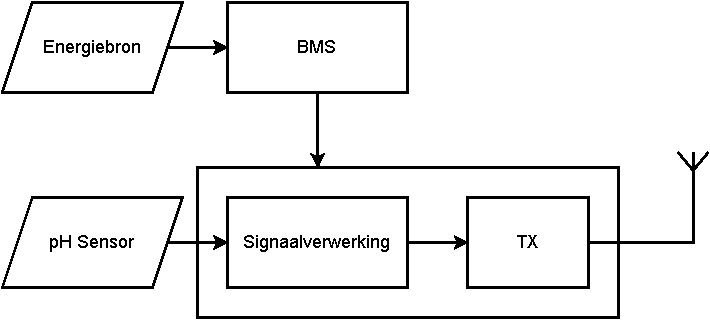
\includegraphics[width=0.6\textwidth]{toplevel}
    \caption{Het volledige systeem.}
    \label{fig:toplevel}
\end{figure}

\subsection{Signaalverwerking}
Het signaalverwerkingsblok maakt een nuttig signaal van de te meten grootheid. Een uitbreiding van dit blok is te zien in \autoref{fig:signaalverwerking}.
Van links naar rechts zijn de functies van de blokken als volgt:
\begin{enumerate}
    \item De grootheid, de pH waarde, wordt gemeten. Dit wordt gedaan door de gate-source spanning $U_{GS}$ van de ISFET te meten.
    \item Het signaal wordt versterkt naar een bruikbare waarde.
    \item Het signaal wordt gefilterd om de bandbreedte te limiteren.
    \item Er wordt voor de kruisgevoeligheid van de pH sensor gecompenseerd d.m.v. een temperatuursensor.
    \item De waarde van $U_{GS}$ wordt omgerekend naar de pH waarde.
    \item Deze waarde wordt draadloos opgestuurd naar de ontvanger.
\end{enumerate}
Het `enable' blok wordt gebruikt om het signaalverwerkingsonderdeel van het systeem te activeren en te deactiveren. Op deze manier hoeft het systeem alleen maar aan te staan wanneer het nodig is, en wordt er minder energie verbruikt. Deze activatie zal waarschijnlijk periodiek gebeuren.

\begin{figure}[ht]
    \centering
    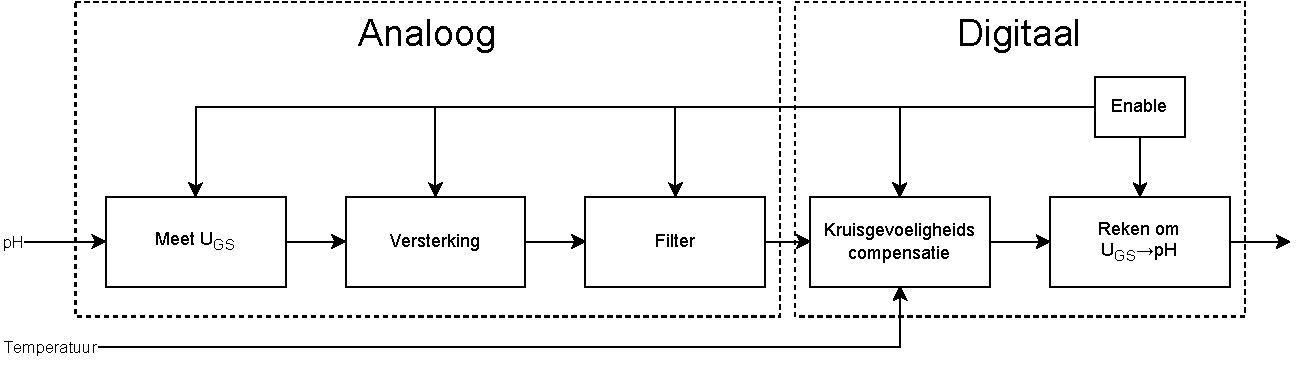
\includegraphics[width=\textwidth]{signaalverwerking}
    \caption{Het signaalverwerkende onderdeel van het systeem, onderverdeeld naar het analoge en digitale domein.}
    \label{fig:signaalverwerking}
\end{figure}

\subsection{BMS}
Het batterijregelingssysteem (BMS) zorgt ervoor dat de batterij opgeladen wordt, terwijl deze ook gebruikt wordt om het systeem te voeden.
De BMS heeft een oplader, die het opladen van de batterij regelt. Deze oplader gaat via een beveiliging naar de batterij toe. De beveiliging zorgt ervoor dat niet te veel stroom en spanning aan de batterij geleverd wordt. De tweede beveiliging zit tussen de batterij en de rest van het systeem. Deze beveiliging zorgt ervoor dat er niet te veel stroom uit de batterij getrokken wordt, waardoor deze kapot kan gaan. De spanningsregelaar zet de spanning die uit de batterij komt om naar een spanning die gebruikt kan worden door de rest van het systeem. 

\begin{figure}[ht]
    \centering
    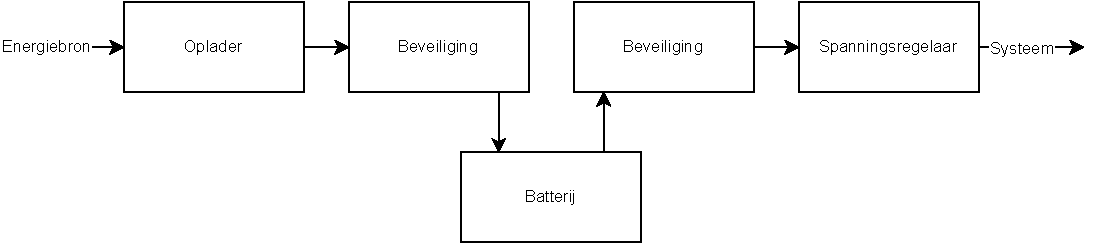
\includegraphics[width=0.9\textwidth]{BMS}
    \caption{Het BMS onderdeel van het systeem.}
    \label{fig:BMS}
\end{figure}

\subsection{TX}
In \autoref{fig:toplevel} is het TX blok het blok dat de data draadloos verstuurt. Dit blok zal direct ingekocht worden; Er zijn namelijk meer dan genoeg kant-en-klare oplossingen beschikbaar om de functie van dit blok te vervullen.


\section{Microcontroller}
Een gedeelte van de signaalverwerking zal gebeuren in het digitale domein. Hiervoor is een microcontroller de voor de hand liggende oplossing. Bij het kiezen van een microcontroller moet er een paar eigenschappen overwogen worden. Een aantal van deze eigenschappen zijn:
\begin{itemize}
    \item gebruikte vermogen;
    \item mogelijke slaapstanden;
    \item beschikbare peripherals;
    \item kloksnelheid;
    \item geheugen;
    \item programmeergeheugen;
    \item en de prijs.
\end{itemize}
